\section{Channel Error Injection Models (ERR\_INJ / AWGN / TAWGN) and HRE}

\begin{frame}{ERR\_INJ: Fixed-Count Random Error Injection}
\vspace{-0.2cm}
\begin{columns}
  \begin{column}{0.56\textwidth}
    \begin{block}{What it models}
      \begin{itemize}
        \item Purpose: emulate a \textbf{fixed error weight} channel where the raw error count is controlled directly.
        \item Input: choose an integer $K$; randomly select $K$ bit positions; flip them deterministically.
        \item Output property: the frame-level error count is fixed: $FBC = K$ (by construction).
        \item This is useful for mapping \textbf{FER vs. error weight} without the randomness of AWGN tails.
      \end{itemize}
    \end{block}
    \begin{block}{How it differs from AWGN}
      \begin{itemize}
        \item No analog amplitude: the channel does not generate a continuous $y$ with noise; it directly flips bits.
        \item No natural reliability distribution: any LLR/quantization derived afterwards is \textbf{not} AWGN-consistent unless explicitly modeled.
      \end{itemize}
    \end{block}
  \end{column}
  \begin{column}{0.40\textwidth}
    \centering
    \begin{tikzpicture}[x=1cm,y=1cm]
      \node[font=\small] at (0,1.35) {Codeword bits ($N$)};
      \draw[rounded corners,fill=gray!10] (-3.1,0.55) rectangle (3.1,1.05);
      \foreach \x/\lbl in {-2.9/0,-2.3/1,-1.7/2,-0.5/\cdots,1.7/N{-}2,2.3/N{-}1} {
        \node[font=\tiny] at (\x,1.12) {\lbl};
      }
      % bit cells
      \foreach \i in {-3,-2.4,-1.8,-1.2,-0.6,0,0.6,1.2,1.8,2.4} {
        \draw[white,line width=0.5pt] (\i,0.55) rectangle (\i+0.55,1.05);
      }
      % mark K error positions
      \foreach \i in {-2.7,-1.5,0.3,2.1} {
        \draw[red,very thick] (\i,0.62) -- (\i+0.45,0.98);
        \draw[red,very thick] (\i+0.45,0.62) -- (\i,0.98);
      }
      \node[font=\small] at (0,0.15) {$K$ random positions flipped};
      \draw[->,thick] (0,-0.1) -- (0,-0.55);
      \node[font=\small] at (0,-0.95) {Fixed $FBC=K$};
    \end{tikzpicture}
  \end{column}
\end{columns}
\end{frame}

\begin{frame}{AWGN: BPSK with Additive Gaussian Noise}
\vspace{-0.2cm}
\begin{columns}
  \begin{column}{0.56\textwidth}
    \begin{block}{Signal model (conceptual)}
      \begin{itemize}
        \item BPSK mapping: bit $b\in\{0,1\}$ maps to $x=-(2b-1)$, so $b=0\to x=+1$ and $b=1\to x=-1$.
        \item Channel: $y=x+\sigma n$ with $n\sim\mathcal{N}(0,1)$ i.i.d.
        \item Hard decision: $\hat b=\mathbf{1}\{y<0\}$; the raw error count $FBC$ is a \textbf{random variable}.
        \item Soft decision: quantize $y$ into bins (by Vref) and look up LLR; reliability comes from distance to decision boundaries.
      \end{itemize}
    \end{block}
    \begin{block}{Why $FBC$ is not fixed}
      \begin{itemize}
        \item Even with fixed $\sigma$, each frame draws a different noise vector, so $FBC$ fluctuates around its mean.
        \item Typical use: estimate FER by Monte Carlo averaging over these naturally occurring fluctuations.
      \end{itemize}
    \end{block}
  \end{column}
  \begin{column}{0.40\textwidth}
    \centering
    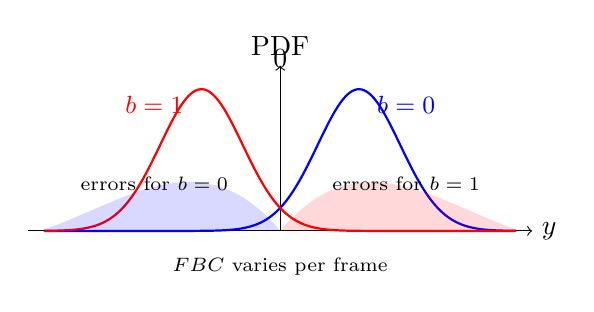
\begin{tikzpicture}[x=1cm,y=1cm]
      \draw[->] (-3.2,0) -- (3.2,0) node[right] {$y$};
      \draw[->] (0,0) -- (0,2.1) node[above] {PDF};
      \draw[dashed] (0,0) -- (0,1.95) node[above] {$0$};
      % two Gaussians (stylized)
      \draw[thick,blue,domain=-3:3,samples=200] plot (\x,{1.8*exp(-(\x-1)^2/0.55)});
      \draw[thick,red,domain=-3:3,samples=200] plot (\x,{1.8*exp(-(\x+1)^2/0.55)});
      \node[blue,font=\small] at (1.6,1.6) {$b=0$};
      \node[red,font=\small] at (-1.6,1.6) {$b=1$};
      % show error regions
      \fill[blue,opacity=0.15] (-3,0) -- (-3,0.02) .. controls (-2.0,0.35) and (-1.0,1.2) .. (0,0) -- cycle;
      \fill[red,opacity=0.15] (0,0) -- (0,0) .. controls (1.0,1.2) and (2.0,0.35) .. (3,0.02) -- (3,0) -- cycle;
      \node[font=\scriptsize] at (-1.6,0.6) {errors for $b=0$};
      \node[font=\scriptsize] at (1.6,0.6) {errors for $b=1$};
      \node[font=\scriptsize] at (0,-0.45) {$FBC$ varies per frame};
    \end{tikzpicture}
  \end{column}
\end{columns}
\end{frame}

\begin{frame}{TAWGN (TRUNC\_AWGN): AWGN Conditioned on Fixed $FBC$}
\vspace{-0.2cm}
\centering
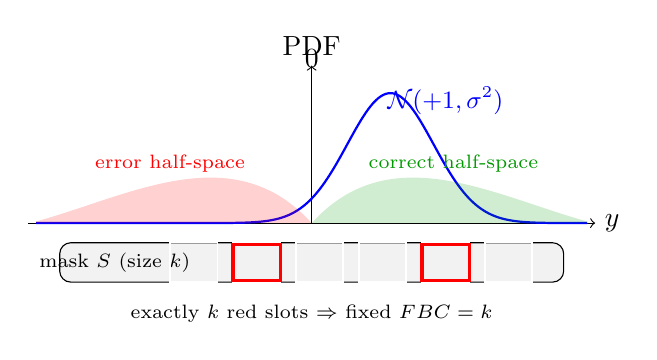
\begin{tikzpicture}[x=1cm,y=1cm]
  % distribution picture (centered)
  \draw[->] (-3.6,0) -- (3.6,0) node[right] {$y$};
  \draw[->] (0,0) -- (0,2.0) node[above] {PDF};
  \draw[dashed] (0,0) -- (0,1.85) node[above] {$0$};
  \draw[thick,blue,domain=-3.5:3.5,samples=220] plot (\x,{1.65*exp(-(\x-1)^2/0.60)});
  \node[blue,font=\small] at (1.7,1.55) {$\mathcal{N}(+1,\sigma^2)$};
  \fill[red,opacity=0.18] (-3.5,0) -- (-3.5,0.02) .. controls (-2.3,0.35) and (-1.0,1.1) .. (0,0) -- cycle;
  \fill[green!60!black,opacity=0.18] (0,0) -- (0,0) .. controls (1.0,1.1) and (2.3,0.35) .. (3.5,0.02) -- (3.5,0) -- cycle;
  \node[red,font=\scriptsize] at (-1.8,0.75) {error half-space};
  \node[green!60!black,font=\scriptsize] at (1.8,0.75) {correct half-space};

  % mask sketch (same slide)
  \draw[rounded corners,fill=gray!10] (-3.2,-0.75) rectangle (3.2,-0.25);
  \node[font=\scriptsize] at (-2.5,-0.50) {mask $S$ (size $k$)};
  \foreach \x in {-1.8,-1.0,-0.2,0.6,1.4,2.2} {
    \draw[white,line width=0.5pt] (\x,-0.75) rectangle (\x+0.6,-0.25);
  }
  \draw[red,very thick] (-1.0,-0.73) rectangle (-0.4,-0.27);
  \draw[red,very thick] (1.4,-0.73) rectangle (2.0,-0.27);
  \node[font=\scriptsize] at (0,-1.15) {exactly $k$ red slots $\Rightarrow$ fixed $FBC=k$};
\end{tikzpicture}

\vspace{-0.05cm}
\begin{itemize}
  \item Goal: generate an AWGN-like frame while enforcing a fixed hard-error count $k$ (per frame).
  \item Method: choose $S$ with $|S|=k$; for $i\in S$ draw $y_i$ from the \textbf{wrong} half-space, else draw from the \textbf{correct} half-space.
  \item Benefit: avoids slow reject-sampling (e.g., \texttt{continue} filters) but still preserves AWGN amplitudes under the condition $FBC=k$.
\end{itemize}
\end{frame}

\begin{frame}{TAWGN $\Leftrightarrow$ Rejection Sampling (1/3): Setup \& Method A}
\vspace{-0.15cm}
\begin{block}{Setup (assume all-zero codeword for clarity)}
\vspace{-0.1cm}
\begin{itemize}
  \item BPSK: transmit $x_i=+1$ and receive $y_i=x_i+n_i$, where $n_i\sim\mathcal{N}(0,\sigma^2)$ i.i.d.
  \item Hard-decision error at position $i$: $\hat b_i=1 \iff y_i<0 \iff n_i<-1$.
  \item Event $E_k$: the frame has exactly $k$ errors, i.e., $\left|\{i: n_i<-1\}\right|=k$.
\end{itemize}
\end{block}

\begin{block}{Method A: rejection sampling (generate then filter)}
\vspace{-0.1cm}
Draw a full noise vector $\bm{n}\sim f(\bm{n})=\prod_{i=1}^{N}\phi_\sigma(n_i)$; accept it only if $\bm{n}\in E_k$:
\[
f_A(\bm{n}) \;=\; f(\bm{n}\mid E_k)
 \;=\; \frac{f(\bm{n})\,\mathbf{1}\{\bm{n}\in E_k\}}{P(E_k)}.
\]
\end{block}
\end{frame}

\begin{frame}{TAWGN $\Leftrightarrow$ Rejection Sampling (2/3): Method B (construction)}
\vspace{-0.15cm}
\begin{block}{Method B: construct samples directly under $E_k$}
\vspace{-0.1cm}
\begin{enumerate}
  \item Choose an error index set $S_{\text{err}}\subset\{1,\dots,N\}$ uniformly at random, with $|S_{\text{err}}|=k$.
  \item For $i\in S_{\text{err}}$: draw $n_i$ from a truncated Gaussian on the \textbf{error} half-space $(-\infty,-1)$.
  \item For $j\notin S_{\text{err}}$: draw $n_j$ from a truncated Gaussian on the \textbf{correct} half-space $[-1,\infty)$.
\end{enumerate}
\end{block}

\begin{block}{Joint PDF of Method B}
\vspace{-0.1cm}
Let $p=P(n<-1)$ be the (single-bit) raw error probability. Then for a given $S_{\text{err}}$,
\[
f(\bm{n}\mid S_{\text{err}})
=
\Big(\prod_{i\in S_{\text{err}}}\frac{\phi_\sigma(n_i)}{p}\Big)
\Big(\prod_{j\notin S_{\text{err}}}\frac{\phi_\sigma(n_j)}{1-p}\Big)
\mathbf{1}\{\bm{n}\in E_k\}.
\]
With uniform set selection $P(S_{\text{err}})=1/\binom{N}{k}$, the unconditional PDF is
\[
f_B(\bm{n})
=
\frac{f(\bm{n})\,\mathbf{1}\{\bm{n}\in E_k\}}
{\binom{N}{k}\,p^k(1-p)^{N-k}}.
\]
\end{block}
\end{frame}

\begin{frame}{TAWGN $\Leftrightarrow$ Rejection Sampling (3/3): Equivalence \& Physical Intuition}
\vspace{-0.15cm}
\begin{columns}
  \begin{column}{0.56\textwidth}
    \begin{block}{Why $f_B(\bm{n})=f_A(\bm{n})$}
    \vspace{-0.15cm}
    \[
    P(E_k)=\binom{N}{k}p^k(1-p)^{N-k}\quad\Rightarrow\quad
    f_B(\bm{n})=\frac{f(\bm{n})\,\mathbf{1}\{\bm{n}\in E_k\}}{P(E_k)}=f(\bm{n}\mid E_k).
    \]
    \vspace{-0.1cm}
    \begin{itemize}
      \item Method A = ``sample then filter'' $\Rightarrow$ conditional distribution $f(\bm{n}\mid E_k)$.
      \item Method B = ``sample directly from $f(\bm{n}\mid E_k)$'' via truncated Gaussians.
      \item Therefore TAWGN (construction) is \textbf{exactly} rejection sampling, but without wasted trials.
    \end{itemize}
    \end{block}
  \end{column}
  \begin{column}{0.40\textwidth}
    \begin{block}{Physical/causal view: why it is valid}
    \vspace{-0.1cm}
    \begin{itemize}
      \item AWGN is \textbf{memoryless}: each $n_i$ only has a value, not a ``generation history''.
      \item Observing ``this bit is wrong'' simply means $n_i$ lies in the error half-space; its posterior is a truncated Gaussian.
      \item The decoder only sees $y$ (or LLR bins). It cannot tell whether $y$ came from filtering or direct construction.
      \item Method A acceptance rate is $P(E_k)$, so expected trials $\approx 1/P(E_k)$ (very slow at high SNR); Method B avoids this.
    \end{itemize}
    \end{block}
  \end{column}
\end{columns}
\end{frame}

\begin{frame}{High-Reliability Error (HRE): Definition and Why It Matters}
\vspace{-0.2cm}
\begin{columns}
  \begin{column}{0.56\textwidth}
    \begin{block}{Definition}
      \begin{itemize}
        \item HRE: a bit that is \textbf{actually wrong} but is reported with \textbf{very high confidence}.
        \item In quantized soft-decision, this corresponds to landing in an \textbf{extreme LLR bin} of the wrong side.
      \end{itemize}
    \end{block}
    \begin{block}{Two common categories}
      \begin{itemize}
        \item Fixed HRE: persistent defects or program/copy failures (bit flips are stable across reads).
        \item Probabilistic HRE: retention/disturb/read-offset tracking issues push some cells deep into the wrong high-confidence region.
      \end{itemize}
    \end{block}
    \begin{block}{Decoder impact (intuition)}
      \begin{itemize}
        \item LDPC relies on soft information; large-magnitude wrong LLRs can dominate message passing and amplify failures.
        \item Measuring both \textbf{FBC} and the \textbf{bin-level breakdown} helps explain when FER is driven by rare high-confidence wrong events.
      \end{itemize}
    \end{block}
  \end{column}
  \begin{column}{0.40\textwidth}
    \centering
    \fbox{\parbox[c][0.62\textheight][c]{0.95\linewidth}{
      \centering
      \textbf{(Figure placeholder)}\\[0.2cm]
      Paste your NAND $V_{th}$ distribution / read-threshold illustration here.
    }}
  \end{column}
\end{columns}
\end{frame}
